\section{La structure task} \label{sec:task}

La structure \texttt{task} (donnée en annexe) est l'abstraction permettant de
définir la notion de \textbf{processus}. Elle porte le même nom dans ALMOS que
dans Linux, et l'équivalent *BSD est la \texttt{struct proc}.  Voici la liste
non exhausitves de toutes les structures contenues ou pointées (la différence
est importante) par la \texttt{struct task}:

  \begin{enumerate}[-]

    \item \texttt{struct task} : le processus doit connaitre son père
        
    \item \texttt{struct cluster\_s} : la structure représentant le cluster sur
      lequel est le processus
    
    \item \texttt{struct cpu\_s} : la structure représentant le cpu sur lequel
      est le processus\footnote{Cette variable serait à supprimer, puisqu'on
      peut avoir l'information via la structure \texttt{cluster\_s}}

    \item \texttt{struct vmm\_s} : le gestionnaire de mémoire virtuel.  Cette
      structure est \textbf{contenue} dans la \texttt{struct task}, \emph{i.e.}
      il n'y a \textbf{pas de pointeurs}

    \item \texttt{struct vfs\_node\_s} : la structure du VFS représentant un
      noeud dans l'arborescence. Ici, le processus connait le noeud racine
      (\textbf{/}) et le répertoire de travail courant

    \item \texttt{struct fd\_info\_s} : cette structure représente les
      descripteurs de fichiers ouverts. On y trouve également la \textbf{table
      de pages}. De même que pour le gestionnaire de mémoire virtuelle, la
      structure \texttt{fd\_info\_s} est \textbf{contenue} par la \texttt{struct
      task}
          
    \item \texttt{struct thread\_s} : cette structure contient tous les threads
      de ce processus.

  \end{enumerate}

  Un processus est donc un ensemble de données permettant de l'identifier
  (\texttt{pid, ppid}), ainsi qu'un ensemble de structures qu'il manipule lors
  de son exécution. Nous allons maintenant nous intéresser à ces structures. On
  donnera le contenu de ces structures de manière non détaillée, en insistant
  sur les points importants.


  \subsection{Les clusters et les processeurs}

    La structure \texttt{cluste\_s} permet une représentation abstraite des
    clusters physique réels de la machine. Un cluster est composé principalement
    des gestionnaires de mémoires, de caches, du tas. On trouve également les
    threads noyaux et les processeurs du cluster.

    Les processeurs sont eux représentés par la structure \texttt{struct
    cpu\_s}.  Ils contiennent l'ordonnanceur, le gestionnaire d'interruption et
    les gestionnaires d'évènements (locaux et distants).

  \subsection{Le gestionnaire de mémoire virtuelle}

    Cette structure est une des plus importante du noyau. C'est elle qui offre
    la vue de la mémoire virtuelle, permettant à chaque processus d'avoir son
    espace d'adressage contigüe (virtuellement), et de penser qu'il est le seul
    sur la machine. Cette structure utilise un gestionnaire de mémoire physique
    (la \texttt{struct pmm\_s}), et pointe également sur une autre structure (la
    \texttt{struct vm\_region\_s} contenant les fonctions relatives à cette
    mémoire virtuelle (\texttt{page\_swap\_in/out()}, \texttt{page\_lookup()},
    \texttt{page\_fault}).

  \subsection{Le VFS}

    Dans un système UNIX, tout est fichier. Ainsi, la manipulation d'information
    pour chaque processus se fera via des fichiers, et donc via le
    VFS\footnote{Virtual File System}. Le VFS est une abstraction du système de
    fichier réel, qui est lui même une abstraction des blocs que composent un
    disque dur. Il fournit un l'API permettant de manipuler les fichiers
    (\texttt{read(), write(), lseek(), mmap() \ldots}). L'implémentation de ces
    fonctions est à la charge du programmeur du système de fichiers.

    L'arborescence même d'un système UNIX est composé de fichiers. En effet, la
    racine "\textbf{/}" est simplement un fichier particulier, contenant les
    informations des fichiers du répertoire. De ce fait, chaque processus a au
    moins deux fichiers ouverts à sa création: la racine, et le répertoire
    courant (\textbf{cwd} pour \textbf{Current Working Directory}).

  \subsection{La table des pages}

    La table des pages est la structure utilisée pour faire le lien entre une
    adresse virtuelle et une adresse physique. Cette structure est donc capable
    de relier une région virtuelle d'un processus, sur un cluster particulier, à
    sa région physique. Pour faire ce calcul, on se base sur l'adresse
    virtuelle, et notamment sur les \textbf{MSB} . Sur la figure \ref{fig:tdp},
    on a pris 20 bits \textbf{MSB}. Ce sont ces derniers que l'on envoi à la
    table et des pages, et qui nous permette de trouver de manière unique la
    page physique associée à cette région virtuelle.
  
    \begin{figure}[!h]
            
        \centering 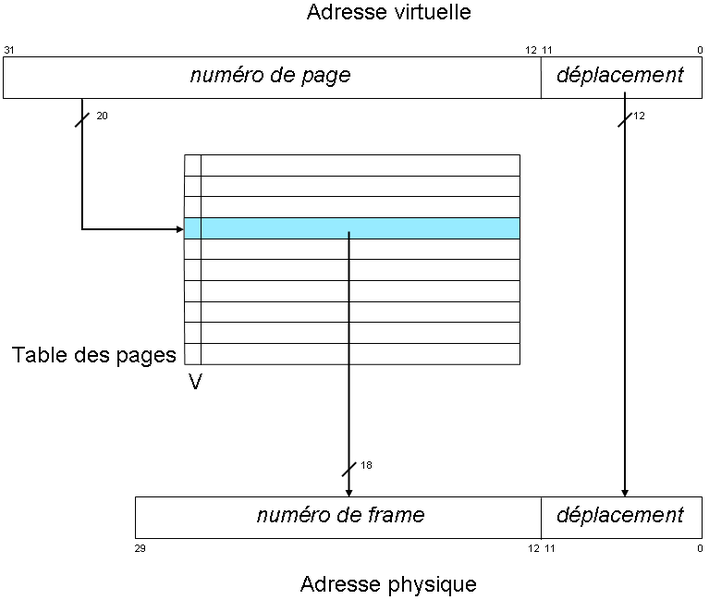
\includegraphics[scale=0.25]{tdp} \caption{Schéma de
        l'opération de traduction d'adresse par la table des pages}
        \label{fig:tdp}
    
    \end{figure}


  \subsection{Les threads}

    Les threads sont les fils d'éxécution du processus. On peut voir un
    processus comme une définition "statique" d'un programme, avec ses pages
    mémoire, les fichiers qu'il accède\ldots, tandis qu'un thread est une
    instance, actuellement en cours d'éxécution, de ce processus.
    
    Un thread est principalement défini par un \texttt{tid} (unique), un
    \texttt{pid} (le même que le processus auquel il appartient), une fonction à
    exécuter, les arguments relatifs à cette fonction, le processeur sur lequel
    il s'éxécute, son contexte d'éxécution et sa pile d'éxécution. L'espace
    d'adressage d'un thread est le même que celui du processus auquel il
    appartient, ce qui signifie que tous les threads d'un même processys
    partagent le même espace d' adressage, et donc que chacun peut voir les
    modifications des autres sur les variables communes. En revanche, les
    variables locales aux threads (celle des fonctions) seront mises dans la
    pile de ce dernier, et seront donc invisible aux autres\footnote{En théorie,
      chaque thread peut accéder aux piles des autres puisqu'ils sont dans le
      même espace d'adressage.  Néanmoins, cette opération est extrêmement
      compliquée puisqu'il faut être capable de trouver l'adresse de début de
    pile du thread que l'on veut "espionner".}.
    
